\section{Indeksy w MySQL}
Indeks jest strukturą danych zwiększającą szybkość operacji wyszukiwania na tabeli. Poprawne stosowanie indeksów jest krytyczne dla zachowania dobrej wydajności bazy danych.
Najprostszą analogią pozwalającą zrozumieć działanie indeksu w bazie danych jest porównanie go z indeksem znajdującym się w książce. Zakładając, że książka nie zawiera indeksu, wyszukiwanie konkretnego słowa lub tematu w najgorszym wypadku wymaga przewertowania całej książki. Z tego powodu w książkach stosuje się indeksy, które zawierają kluczowe słowa użyte w książce. Indeks taki zawiera listę słów oraz stron, na których słowa te występują. Dzięki temu wyszukanie konkretnego słowa wymaga jedynie sprawdzenia numeru strony w indeksie. Jest to szczególnie przydatne przy książkach zawierających dużą liczbę stron. Podobnie jest z tabelami w bazie danych. Przy tabelach o niewielkiej ilości wierszy, wyszukanie konkretnego rekordu trwa krótki nawet przy niestosowaniu indeksów. Indeksy stają się jednak kluczowe wraz ze wzrostem zbioru danych.
W MySQL istnieje wiele rodzajów indeksów, które są implementowane w wartstwie silnika bazy danych, dlatego też nie każdy rodzaj indeksu jest obsługiwany przez wszystkie silniki. W tym rozdziale omówię tylko najpopularniejsze z nich.
\subsection{Indeksy typu B-Tree}
Indeks typu B-Tree jest zdecydowanie najczęściej stosowanym typem indeksu w bazach MySQL i jest domyślnie wybierany przez serwer MySQL podczas tworzenia nowego indeksu. Dlatego właśnie jemu poświęce zdecydowaną wiekszość tego rozdziału.

\paragraph{Struktura}\mbox{}

Indeks typu B-Tree zbudowany jest na bazie struktury B-Drzewa. B-Drzewo jest drzewiastą strukturą danych przechowującą dane wraz z kluczami posortowanymi w pewnej kolejności. Każdy węzeł drzewa może posiadać od M+1 do 2M+1 dzieci, za wyjątkiem korzenia, który od 0 do 2M+1 potomków, gdzie M jest nazywany rzędem drzewa. Dzięki temu maksymalna wysokość drzewa zawierającego n kluczy wynosi $log_M n$. Takie właściwości sprawiają, że operacje wyszukiwania są złożoności asymptotycznej $O(log_M n)$. Chcąc być dokładnym, należy wspomnieć, że MySQL do zapisu indeksów stosuje strukurę B+Drzewa, która jest szczególnym przypadkiem B-Drzewa i zawiera dane jedynie w liściach.
Zastosowanie struktury B+Drzewa sprawia, że liście z danymi znajdują się w jednakowej odległości od korzenia drzewa. Wysoki rząd oznacza niską wysokość drzewa, to z kolei sprawia, że zapytanie wymaga mniejszej ilości operacji odczytu z dysku. Ma to fundamentalne znaczenie, ponieważ dane zapisane są na dyskach twardych, których czasy dostępu są dużo większe niż do pamięci RAM. Dla przykładu, załóżmy, że dana jest tabela zawierająca bilion wierszy, oraz indeks, którego rząd wynosi 64. Operacja wyszukania na danej tabeli wykorzystująca indeks będzie wymagać średnio tylu operacji odczytu, jaka jest wysokość drzewa przechowującego indeksy. Wysokość drzewa obliczamy ze wzoru $\log M n$,gdzie M jest rzędem drzewa równym 64, a n oznacza ilość wierszy. W takim przypadku będziemy potrzebować zaledwie 5 odczytów danych z dysku. Dodatkowo silnik InnoDB nie przechowuje referencji do miejsca w pamięci, w którym znajdują się dane, ale odwołuje się do rekordów poprzez klucz podstawowy, który jednoznacznie identyfikuje każdy wiersz w tabeli.Dzięki temu zmiana fizycznego położenia rekordu nie wymusza aktualizacji indeksu. Indeksy mogą być zakładane zarówno na jedną jak i wiele kolumn. W przypadku indeksu wielokolumnowego, węzły sortowane są w pierwszej kolejności względem pierwszej kolumny indeksu. W następnej kolejności węzły z równymi wartościami pierwszej kolumny, sortowane są względem drugiej itd. Kolejność kolumn jest ustalana na podstawie kolejności podczas polecenia tworzenia indeksu.

\paragraph{Zastosowanie indeksu typu B-Tree}\mbox{}

Aby przedstawić działanie indeksu typu B-Tree na rzeczyczywistym przykładzie przygotowałem dwie tabele. Pierwszą jest tabela \textit{Comments} z bazy danych stackoverflow. Drugą tabelą jest \textit{Init\textunderscore Comments}, która jest kopią tabeli Comments i nie zawiera klucza głównego oraz indeksów.
Dla tabeli \textit{Comments\textunderscore idx} za pomocą polecania \begin{verbatim}
    CREATE INDEX user_post_idx 
ON Comments(UserId,PostId);
\end{verbatim}
utworzyłem indeks typu B-Tree na dwóch kolumnach \textit{first\textunderscore UserId} oraz \textit{last\textunderscore PostId}.

\subparagraph{Dopasowanie pełnego indeksu}\mbox{}

Załóżmy, że w tabeli \textit{Comments} chcemy wyszukać wszystkie komentarze użytkownika o id 1200 do postu o id 910331.

Najpierw wykonamy zapytania na tabeli nie zawierającej indeksów.
 \textit{employees}. 
\begin{verbatim}
    SELECT * FROM Init_Comments WHERE UserId = 1200 AND PostId = 910331;
\end{verbatim}
Zapytanie zwróciło wynik w 13,7 sekundy.

Następnie analogiczne zapytanie wykonałem na tabeli \textit{Comments} zawierającej indeks na obu kolumnach.
\textit{employees\textunderscore idx}. 
\begin{verbatim}
    SELECT * FROM Comments WHERE UserId = 1200 AND PostId = 910331;
\end{verbatim}
Tym razem zapytanie zwróciło wyniki w 0,013 sekundy. Tym razem serwer nie skanował całej tabeli. Z czego wynika różnica w czasie wykonania obu zapytań? Wykorzystując polecenie EXPLAIN dla obu zapytań otrzymujemy ciekawe dane. Rysunek 2 przestawia wynik polecenia EXPLAIN dla pierwszego zapytania, natomiast Rysunek 3 wynik polecania EXPLAIN dla drugiego zapytania. Polecenie EXPLAIN wyjaśnia, że pierwsze zapytania nie będzie korzystać z indeksów, dlatego w kolumnie rows widzimy, że serwer MySQL będzie musiał przeskanować wszystkie 23 miliony wierszy z tabeli \textit{init\textunderscore Comments}. Drguie zapytanie korzysta z indeksu z naszego indeksu. Tym razem serwer będzie musiał przeskanować jedynie 3 wiersze tabeli Comments. 

\begin{figure}[h]
    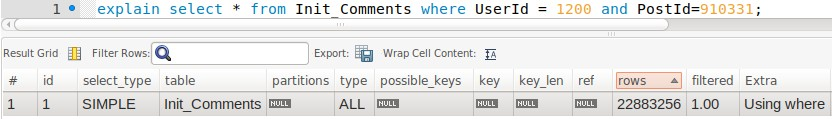
\includegraphics[scale =0.5]{explain1.jpg} 
    \caption{EXPLAIN 1}
\end{figure}

\begin{figure}[h]
    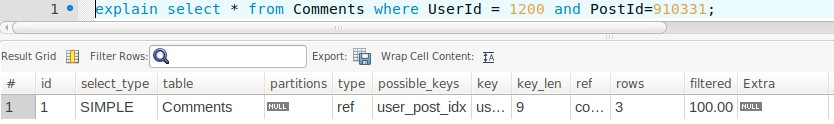
\includegraphics[scale =0.5]{explain2.jpg} 
    \caption{EXPLAIN 2}
\end{figure}

Dopasowanie pełnego indeksu ma miejsce wtedy, kiedy w klauzuli \textit{where} uwzględnimy wszystkie kolumny, na które założony jest indeks. 
\subparagraph{Dopasowanie prefiksu znajdującego się najbardziej na lewo}\mbox{} 
Dopasowanie prefiksu znajdującego się najbardziej na lewo może pomóc w wyszukaniu wsystkich komentarzy użytkownika. Załóżmy, że chcemy znaleźć wszystkie komentarze użytkownika o id 1200.
W tym celu przygotowujemy dwa zapytania. Pierwsze na tabeli \textit{Init\textunderscore Comments}, drugie na tebeli \textit{Comments} zawierającej indeks typu B-Tree, który założyliśmy wcześniej.
\begin{verbatim}
    SELECT * FROM Init_Comments WHERE UserId = 1200;
\end{verbatim}
\begin{verbatim}
    SELECT * FROM Comments WHERE UserId = 1200;
\end{verbatim}
Pierwsze zapytanie zostało wykonane w czasie 12,9 sekundy, natomiast drugie wymagało jedynie 0,0044 sekundy. Ponownie sprawdźmy rezultat polecenia EXPLAIN na obu zapytaniach. W pierwszym zapytaniu serwer po raz kolejny musiał przeszukać wszystkie wiersze w tabeli. Drugie zapytanie wymagało przeszukania 209 wierszy, dlatego że tym razem zapytanie było mniej selektywne niż przy dopasowaniu pełnego indeksu.
\begin{figure}[h]
    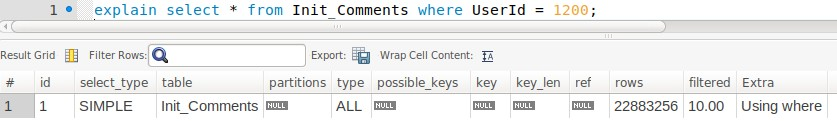
\includegraphics[scale =0.5]{explain3.jpg} 
    \caption{EXPLAIN 3}
\end{figure}

\begin{figure}[h]
    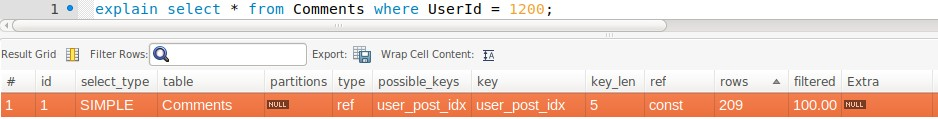
\includegraphics[scale =0.5]{explain4.jpg} 
    \caption{EXPLAIN 4}
\end{figure}

\subparagraph{Dopasowanie zakresu wartości}\mbox{}
Dopasowanie zakresu wartości oznacza wyszukiwanie wartości w danym przedziale. W naszym przypadku może to być wyszukiwanie wszystkich komentarzy użytkowników o identyfikatorach z przedziału od 1990 do 2000.

Ponownie wykonujemy dwa zapytania. Pierwsze na tabeli bez indeksu, drugie na tabeli z indeksem.
\begin{verbatim}
    SELECT * FROM Init_Comments WHERE UserId >1990 AND UserId <2000;
\end{verbatim}

Tym razem pierwsze zapytanie trwało 1.068 sekundy. Drugie zapytanie wykonujemy na tabeli Comments zawierającej indeksy.
\begin{verbatim}
    SELECT * FROM Comments WHERE UserId >1990 AND UserId <2000;
\end{verbatim}
Następnie sprawdzamy wynik polecenia EXPLAIN dla obu zapytań. Przy pierwszym zapytaniu, kolejny raz MySQL przeskanował całą tabelę Init\textunderscore Comments. Drugie natomiast wymagało przeskanowania jedynie wierszy, które zostały zwrócone jako rezultat zapytania.

\begin{figure}[h]
    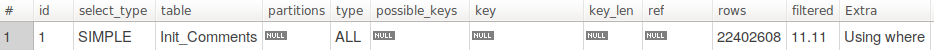
\includegraphics[scale =0.5]{explain5.png} 
    \caption{EXPLAIN 5}
\end{figure}

\begin{figure}[h]
    
\includegraphics[scale =0.5]{explain6.png} 
    \caption{EXPLAIN 6}
\end{figure}


PREFIX INDEX
będą wymagały przeszukania całej tabeli. Dodatkowo wyszukiwanie za pomocą prefiksu nie będzie optymalne w przypadku indeksu wielokolumnowego dla wszystkich kolumn z wyjątkiem pierwszej. Jest to bezpośrednim następstwem budowy indeksów typu B-Tree i wynika z faktu sortowania kluczy względem pierwszej kolumny.





\subparagraph{Zapytania dotyczące jedynie indeksów}\mbox{}
Zapytania dotyczące jedynie indeksów to zapytania, które wykorzystują jedynie wartości indeksu, a nie do rekordów bazy danych.





 
Indeks jednokolumnowy zawiera klucze posortowane zgodnie z wartościami kolumny, na której założony został indeks. W przypadku indeksów wielokolumnowych węzły sortowane są w kolejności kolumn w indeksie. Zakładając, że indeks został założony na kolumnach k1,k2 oraz k3, dane w pierwszej kolejności zostaną posortowane zgodnie z wartościami kolumny k1. Następnie rekordy z równą wartością kolumny k1 zostaną posortowane zgodnie z wartościami kolumny k2. Analogicznie rekordy z równą wartością kolumny k1 oraz k2 zostaną posortowane zgodnie z wartościami kolumny k3. Zrozumienie tej zasady jest kluczowe do poprawnego korzystania z indeksów typu B-Tree. Taka struktura powoduje, że taki indeks jest użyteczny tylko w przypadku, gdy wyszukiwanie używa znajdujego się najbardziej na lewo prefiksu indeksu.
Kolejnym zastosowaniem indeksu typu B-Tree jest wyszukiwanie na podstawie prefiksu kolumny. Przykładem takiego zapytania może być wyszukiwanie wszystkich pracowników, których nazwiska rozpoczynają się od litery K (zakładamy, że tabela posiada indeks na kolumnie nazwisko). Istotnym jest fakt, że indeks staje się nieprzydany przy wyszukiwaniu na podstawie suffixu lub środkowej wartości. Następnym przypadkiem, w którym indeks typu B-Tree przyśpiesza zapytanie, jest wyszukiwanie na podstawie zakresu wartości. Dla tabeli z indeksem typu B-Tree założonym na kolumnie k, indeks może posłużyć do efektywnego wyszukania wartości z przedziału wartości tej kolumny. Zastosowanie struktury B-Tree powoduje, że sortowanie wyników zapytania względem indeksy jest zdecydowanie bardziej wydajne.


\subsection{Indeksy typu hash}
Indeksy typu hash są dostępne jedynie dla tabel silnika \textit{MEMORY} i są domyślnie ustawianymi indeksami dla takich tabel. Indeksy typu \textit{hash} opierają się na funkcji skrótu liczonej na wartościach indeksowanych kolumn. Dla każdego rekordu takiej tabeli liczona jest krótka sygnatura, na podstawie wartości klucza wiersza. Podczas wyszukiwania wartości na podstawie kolumn indeksowanych tego typu kluczem obliczana jest funkcja skrótu dla klucza, a następnie wyszukuje w indeksie odpowiadających wierwszy. Możliwe jest, że do jednej wartości funkcji skrótu dopasowane zostanie więcej niż jeden różny wiersz. Takie zachowanie wynika bezpośrednio z zasady działania funkcji skrótu, która nie zapewnia unikatowości dla różnych wartości dla zbioru danych wejściowych. Niemniej taka sytuacja nie należy do częstych i nawet wtedy operacja wyszukiwania na podstawie indeksu typu hash jest bardzo wydajna, ponieważ serwer w najgorszym wypadku musi odczytać zaledwie kilka wierszy z tabeli. Stąd wynika największa zaleta indeksów typu \textit{hash} w stosunktu do indeksów \textit{B-Tree}; czas wyszukiwania dowolnego wiersza w tabeli jest stały niezależnie od liczby wierszy. Podstawową wadą indeksu typu hash jest konieczność wyszukiwania na podstawie pełnej wartości klucza. Wynika to z tego, że funkcja skrótu wyliczona na podstawie niepełnego zbioru danych, nie ma korelacji z wartością funkcji wyliczonej na pełnym kluczu. Dodatkowo indeksy hash nie optymalizują operacji sortowania, ponieważ wartości funkcji f1, f2 skrótu dla dwóch rekordów x1 oraz x2, gdzie x1 jest mniejsze od x2 nie zapewniają, że f1 będzie mniejsze od f2. Dodatkowo z racji ograniczonego zbioru wartości funkcji hashującej, mogą występować problemy ze skalowaniem w przypadku dużych zbiorów danych. Po przekroczeniu pewnej liczby wierszy, należy zwiększyć rozmiar klucza indeksu i ponownie obliczyć funkcję dla wszystkich wierszy w tabeli.

